% =====================================================================
% BMED365 (Spring 2027) — Lab 5: The Computational Kiwi Challenge
% Companion Guide (Part 2): Polyploid Stability, 3D Point Processes,
%                           Inverse Problems & 3D Bloch-MRI Digital Twin
% Compile with: pdflatex inverse-problems-and-digital-twin.tex (run twice)
% =====================================================================
\documentclass[10.5pt,a4paper]{article}

\usepackage[utf8]{inputenc}
\usepackage[T1]{fontenc}
\usepackage[english]{babel}
\usepackage{lmodern}
\usepackage{microtype}
\usepackage{graphicx}
\usepackage{booktabs}
\usepackage{tabularx}
\usepackage{array}
\usepackage{colortbl}
\usepackage{xcolor}
\usepackage{amsmath,amssymb}
\usepackage{enumitem}
\usepackage[margin=1.9cm,headheight=14pt]{geometry}
\usepackage{fancyhdr}
\usepackage{titlesec}
\usepackage[most]{tcolorbox}
\usepackage{listings}
\usepackage{float}
\usepackage{tikz}
\usetikzlibrary{arrows.meta,positioning,shapes.geometric,fit,backgrounds,calc}
\usepackage{hyperref}

% =====================================================================
% COLORS & HYPERREF (UiB / BMED365 House Style)
% =====================================================================
\definecolor{uibblue}{RGB}{0, 61, 115}
\definecolor{uibred}{RGB}{175, 28, 44}
\definecolor{kiwigreen}{RGB}{27, 138, 90}
\definecolor{amberwarn}{RGB}{195, 110, 0}
\definecolor{lightgray}{RGB}{246, 248, 250}
\definecolor{rowalt}{RGB}{242, 246, 251}
\definecolor{codebg}{RGB}{248, 249, 251}
\definecolor{codekw}{RGB}{0, 75, 145}
\definecolor{codestr}{RGB}{155, 35, 45}
\definecolor{codecmt}{RGB}{95, 105, 115}

\hypersetup{
    colorlinks=true,
    linkcolor=uibblue,
    citecolor=uibblue,
    urlcolor=uibred,
    pdftitle={Computational Modeling of the Kiwifruit (Part 2): Inverse Problems & 3D Bloch-MRI Digital Twin (BMED365 Spring 2027)},
    pdfauthor={Arvid Lundervold (UiB / MMIV) -- BMED365 Spring 2027}
}

% =====================================================================
% TYPOGRAPHY, HEADERS & CALLOUT BOXES
% =====================================================================
\setlength{\parindent}{0pt}
\setlength{\parskip}{0.45em}
\setlist[itemize]{topsep=2pt,itemsep=2pt,leftmargin=1.4em}
\setlist[enumerate]{topsep=2pt,itemsep=2pt,leftmargin=1.6em}

\newcolumntype{L}[1]{>{\raggedright\arraybackslash}p{#1}}
\newcolumntype{C}[1]{>{\centering\arraybackslash}p{#1}}
\newcolumntype{R}[1]{>{\raggedleft\arraybackslash}p{#1}}
\newcolumntype{Y}{>{\raggedright\arraybackslash}X}

\titleformat{\section}{\Large\bfseries\color{uibblue}}{\thesection}{0.7em}{}[\vspace{1pt}\titlerule]
\titleformat{\subsection}{\large\bfseries\color{uibblue!88!black}}{\thesubsection}{0.6em}{}
\titleformat{\subsubsection}{\normalsize\bfseries\color{uibblue!75!black}}{\thesubsubsection}{0.5em}{}
\titlespacing*{\section}{0pt}{1.15em}{0.45em}
\titlespacing*{\subsection}{0pt}{0.85em}{0.3em}

\pagestyle{fancy}
\fancyhf{}
\fancyhead[L]{\footnotesize\textcolor{gray}{BMED365 (Spring 2027) $\cdot$ Lab 5: Computational Kiwi Challenge (Part 2)}}
\fancyhead[R]{\footnotesize\textcolor{gray}{Inverse Problems \& 3D Bloch-MRI Digital Twin}}
\fancyfoot[L]{\footnotesize\textcolor{gray}{University of Bergen \& MMIV $\cdot$ CC BY-SA 4.0}}
\fancyfoot[R]{\footnotesize\textcolor{gray}{Page \thepage}}
\renewcommand{\headrulewidth}{0.4pt}
\renewcommand{\footrulewidth}{0.2pt}

\newtcolorbox{infobox}[1][]{
    enhanced,
    colback=lightgray, colframe=uibblue,
    fonttitle=\bfseries\small, title=#1,
    boxrule=0.6pt, arc=2.5pt, left=7pt, right=7pt, top=5pt, bottom=5pt
}

\newtcolorbox{warningbox}[1][]{
    enhanced,
    colback=uibred!4, colframe=uibred,
    fonttitle=\bfseries\small, title=#1,
    boxrule=0.6pt, arc=2.5pt, left=7pt, right=7pt, top=5pt, bottom=5pt
}

\newtcolorbox{qabox}[1][]{
    enhanced,
    colback=kiwigreen!5, colframe=kiwigreen!85!black,
    fonttitle=\bfseries\small, title=#1,
    boxrule=0.6pt, arc=2.5pt, left=7pt, right=7pt, top=5pt, bottom=5pt
}

\lstdefinestyle{pybmed}{
    language=Python,
    backgroundcolor=\color{codebg},
    basicstyle=\ttfamily\scriptsize,
    keywordstyle=\bfseries\color{codekw},
    stringstyle=\color{codestr},
    commentstyle=\itshape\color{codecmt},
    showstringspaces=false,
    breaklines=true,
    breakatwhitespace=true,
    frame=single,
    rulecolor=\color{uibblue!30},
    framesep=4pt,
    xleftmargin=3pt,
    xrightmargin=3pt,
    columns=fullflexible,
    keepspaces=true,
    upquote=true
}

% =====================================================================
% DOCUMENT START
% =====================================================================
\begin{document}

% Title Banner
\begin{tcolorbox}[enhanced, colback=uibblue!6, colframe=uibblue, boxrule=1.0pt, arc=3pt, left=10pt, right=10pt, top=9pt, bottom=9pt]
{\LARGE\bfseries\color{uibblue} Computational Modeling of the Kiwifruit (Part 2)}\\[3pt]
{\normalsize\bfseries Polyploid Stability, 3D Spatial Point Processes, Ill-Posed Inverse Problems \& a 3D Bloch-MRI Digital Twin}\\[3pt]
{\small \textbf{Course:} BMED365 --- Computational Imaging, Modeling and AI in Biomedicine (Spring 2027), University of Bergen \& MMIV\\
\textbf{Coordinator:} Arvid Lundervold \quad$\cdot$\quad \textbf{Environment:} Pure CPU (\texttt{NumPy}/\texttt{SciPy}/\texttt{scikit-image}; \texttt{bmed365-2027} \texttt{uv} \& Google Colab)\\[3pt]
\textbf{Companion Resources:} \href{https://github.com/arvidl/BMED365-2027/blob/main/Lab5-Comp-Mod/Kiwi-challenge/notebooks/02-kiwi-digital-twin-and-inverse-problems.ipynb}{Notebook \texttt{02} (GitHub)} $\;\vert\;$ \href{https://colab.research.google.com/github/arvidl/BMED365-2027/blob/main/Lab5-Comp-Mod/Kiwi-challenge/notebooks/02-kiwi-digital-twin-and-inverse-problems.ipynb}{Open NB \texttt{02} in Colab} $\;\vert\;$ \href{https://github.com/arvidl/BMED365-2027/blob/main/Lab5-Comp-Mod/Kiwi-challenge/docs/inverse-problems-and-digital-twin.md}{Markdown} $\;\vert\;$ \href{https://github.com/arvidl/BMED365-2027/blob/main/Lab5-Comp-Mod/Kiwi-challenge/docs/foundations-atlas-and-morphogenesis.pdf}{Part~1 PDF}}
\end{tcolorbox}

\vspace{-2pt}
{\small\tableofcontents}
\vspace{4pt}
\hrule
\vspace{6pt}

% =====================================================================
% SECTION 1: NON-TECHNICAL INTRODUCTION & VISUAL INTUITION
% =====================================================================
\section{A Non-Technical Introduction: Big Ideas, Definitions \& Visual Intuition}

\begin{infobox}[Who This Section Is For (Start Here!)]
Part~2 tackles four pillars of quantitative computational medicine: \textbf{stability analysis}, \textbf{3D spatial statistics}, \textbf{ill-posed inverse problems}, and \textbf{physics-based Digital Twins}. Before introducing eigenvalues, singular values, or Bloch equations, this opening section translates every idea into plain English and visual intuition --- designed for biomedicine master's students with moderate math background.
\end{infobox}

\subsection{From Forward Simulation to Inverse Detective Work \& Virtual Phantoms}

In \href{https://github.com/arvidl/BMED365-2027/blob/main/Lab5-Comp-Mod/Kiwi-challenge/docs/foundations-atlas-and-morphogenesis.pdf}{\textbf{Part~1}}, we ran biology \textbf{forward}: starting from genes, seeds, and hormones, we simulated a kiwifruit growing to $86\text{ cm}^3$ with 33 radial chambers. Yet modern computational medicine demands four deeper questions that Part~2 answers directly on our 2005 7\,T MRI dataset:

\begin{enumerate}
    \item \textbf{``Why does doubling or tripling genome size change the number of organ chambers?''} Wild diploid ($2x$) golden kiwifruit have $\sim 22$ radial chambers, whereas our hexaploid ($6x$) green \texttt{'Hayward'} berry has $33$. Instead of running endless trial-and-error simulations, \textbf{linear stability analysis} lets us predict the winning chamber count directly --- the exact math explaining why widening an embryonic limb bud causes \emph{polydactyly} (extra fingers)!
    \item \textbf{``Are the seeds scattered at random, or do they obey hidden 3D spatial architecture?''} Using the 98 curated 3D seeds from Lab~4, \textbf{3D spatial point-process statistics} prove that seeds maintain a strict ``personal space'' ($\sim 0.95\text{ mm}$) at short range while aligning into radial rows at medium range --- the exact same spatial statistics used in \textbf{Lab~4 Imaging Mass Cytometry (\texttt{IMC})} to quantify whether \texttt{CD8+} T cells infiltrate or are excluded from a tumor!
    \item \textbf{``Can we run physics \emph{backward} to diagnose hidden interior damage from outside measurements?''} Suppose we can measure only the smooth outer skin contour of a fruit (or only chest-surface \texttt{ECG} electrodes / scalp \texttt{EEG} electrodes in a patient) and want to reconstruct hidden internal deficits. Running blurring backward naively causes tiny measurement noise to explode by \textbf{470,000\%}! \textbf{Tikhonov regularization} adds a ``smoothness seatbelt'' that recovers the hidden cause to within \textbf{5\% error}.
    \item \textbf{``How can we prove an AI segmentation pipeline works when nobody dissected the 2005 fruit?''} We close the \textbf{Lab~5 $\to$ Lab~4 Digital Twin loop}: we build a \textbf{virtual 3D kiwifruit} with an exact known seed count ($N_{\text{true}} = 750$), simulate a real 7\,T Bruker scanner (including authentic \textbf{Rician MRI noise}), run Lab~4's 3D detector on it, and candidly audit the \textbf{Sim-to-Real Gap} between synthetic phantoms and messy biological reality!
\end{enumerate}

\subsection{Visual Intuition: Four Advanced Concepts Made Visual}

\begin{figure}[H]
\centering
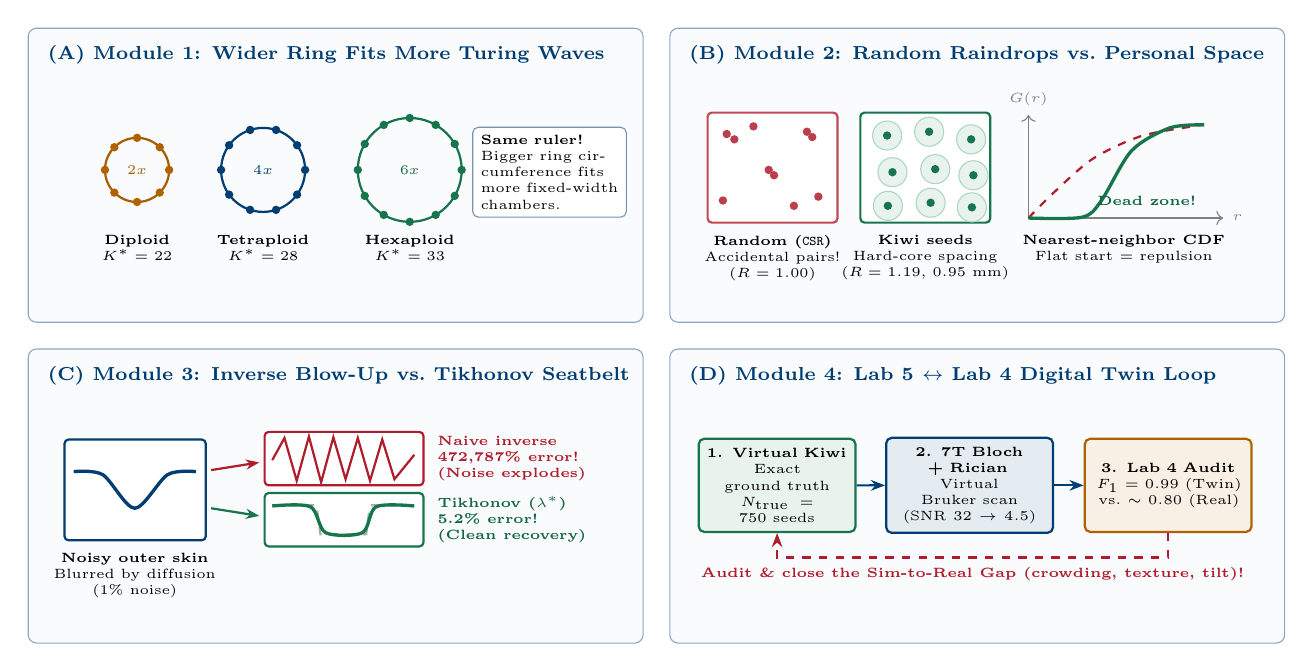
\begin{tikzpicture}[
    scale=0.97, transform shape,
    font=\scriptsize,
    panel/.style={rectangle, rounded corners=3pt, draw=uibblue!45, fill=lightgray!55, inner sep=4pt, minimum width=8.05cm, minimum height=3.85cm}
]
% --- PANEL A: Polyploid Ring Quantization ---
\node[panel] (pA) at (0,0) {};
\node[anchor=north west, font=\scriptsize\bfseries\color{uibblue}] at ([xshift=4pt,yshift=-3pt]pA.north west) {(A) Module 1: Wider Ring Fits More Turing Waves};

\begin{scope}[shift={(-3.55,-1.08)}]
    % 2x ring
    \draw[amberwarn!85!black, thick] (0.95,1.15) circle (0.42);
    \foreach \k in {0,45,90,135,180,225,270,315}{
        \fill[amberwarn!90!black] ({0.95+0.42*cos(\k)},{1.15+0.42*sin(\k)}) circle (0.055);
    }
    \node[font=\tiny\bfseries, color=amberwarn!85!black] at (0.95,1.15) {$2x$};
    \node[below, align=center, font=\tiny] at (0.95,0.42) {\textbf{Diploid}\\$K^* = 22$};

    % 4x ring
    \draw[uibblue, thick] (2.60,1.15) circle (0.55);
    \foreach \k in {0,36,72,108,144,180,216,252,288,324}{
        \fill[uibblue] ({2.60+0.55*cos(\k)},{1.15+0.55*sin(\k)}) circle (0.055);
    }
    \node[font=\tiny\bfseries, color=uibblue] at (2.60,1.15) {$4x$};
    \node[below, align=center, font=\tiny] at (2.60,0.42) {\textbf{Tetraploid}\\$K^* = 28$};

    % 6x ring
    \draw[kiwigreen!85!black, thick] (4.52,1.15) circle (0.68);
    \foreach \k in {0,30,60,90,120,150,180,210,240,270,300,330}{
        \fill[kiwigreen!85!black] ({4.52+0.68*cos(\k)},{1.15+0.68*sin(\k)}) circle (0.055);
    }
    \node[font=\tiny\bfseries, color=kiwigreen!75!black] at (4.52,1.15) {$6x$};
    \node[below, align=center, font=\tiny] at (4.52,0.42) {\textbf{Hexaploid}\\$K^* = 33$};

    \node[rectangle, rounded corners=2pt, draw=uibblue!55, fill=white, align=left, font=\tiny, text width=1.80cm, inner sep=3pt] at (6.35,1.12) {\textbf{Same ruler!}\\Bigger ring circumference fits more fixed-width chambers.};
\end{scope}

% --- PANEL B: CSR vs Personal Space ---
\node[panel] (pB) at (8.40,0) {};
\node[anchor=north west, font=\scriptsize\bfseries\color{uibblue}] at ([xshift=4pt,yshift=-3pt]pB.north west) {(B) Module 2: Random Raindrops vs.\ Personal Space};

\begin{scope}[shift={(4.82,-1.08)}]
    % Random CSR box
    \fill[white, draw=uibred!80, thick, rounded corners=1.5pt] (0.05,0.46) rectangle (1.75,1.90);
    \foreach \x/\y in {0.30/1.62, 0.40/1.55, 1.35/1.65, 1.42/1.58, 0.85/1.15, 0.92/1.08, 0.25/0.75, 1.50/0.80, 1.18/0.68, 0.65/1.72}{
        \fill[uibred!85] (\x,\y) circle (0.055);
    }
    \node[below, align=center, font=\tiny] at (0.90,0.42) {\textbf{Random (\texttt{CSR})}\\Accidental pairs!\\($R = 1.00$)};

    % Hard-core spaced box
    \fill[white, draw=kiwigreen!85!black, thick, rounded corners=1.5pt] (2.05,0.46) rectangle (3.75,1.90);
    \foreach \x/\y in {0.35/1.60, 0.90/1.65, 1.45/1.55, 0.42/1.12, 0.98/1.16, 1.48/1.08, 0.36/0.68, 0.92/0.72, 1.46/0.66}{
        \draw[kiwigreen!35, fill=kiwigreen!10] ({2.05+\x},\y) circle (0.19);
        \fill[kiwigreen!85!black] ({2.05+\x},\y) circle (0.055);
    }
    \node[below, align=center, font=\tiny] at (2.90,0.42) {\textbf{Kiwi seeds}\\Hard-core spacing\\($R = 1.19$, $0.95\text{ mm}$)};

    % G(r) curve
    \begin{scope}[shift={(4.25,0.52)}]
        \draw[->, thin, gray] (0,0) -- (2.55,0) node[right, font=\tiny] {$r$};
        \draw[->, thin, gray] (0,0) -- (0,1.35) node[above, font=\tiny] {$G(r)$};
        \draw[uibred, thick, dashed] plot[smooth] coordinates {(0,0) (0.35,0.35) (0.85,0.78) (1.50,1.08) (2.30,1.22)};
        \draw[kiwigreen!85!black, very thick] plot[smooth] coordinates {(0,0) (0.70,0.01) (0.95,0.22) (1.35,0.88) (1.85,1.18) (2.30,1.22)};
        \node[font=\tiny\bfseries, color=kiwigreen!75!black] at (1.55,0.22) {Dead zone!};
        \node[below, align=center, font=\tiny] at (1.25,-0.10) {\textbf{Nearest-neighbor CDF}\\Flat start = repulsion};
    \end{scope}
\end{scope}

% --- PANEL C: Frosted Glass Inverse Blow-up ---
\node[panel] (pC) at (0,-4.20) {};
\node[anchor=north west, font=\scriptsize\bfseries\color{uibblue}] at ([xshift=4pt,yshift=-3pt]pC.north west) {(C) Module 3: Inverse Blow-Up vs.\ Tikhonov Seatbelt};

\begin{scope}[shift={(-3.55,-5.28)}]
    % Smooth blurry measurement
    \fill[white, draw=uibblue, thick, rounded corners=1.5pt] (0,0.50) rectangle (1.85,1.82);
    \draw[uibblue, very thick] plot[smooth] coordinates {(0.12,1.40) (0.50,1.36) (0.92,0.92) (1.35,1.36) (1.72,1.40)};
    \node[below, align=center, font=\tiny] at (0.92,0.46) {\textbf{Noisy outer skin}\\Blurred by diffusion\\(1\% noise)};

    \draw[-{Stealth[length=1.7mm]}, thick, color=uibred] (1.92,1.42) -- (2.55,1.52);
    \draw[-{Stealth[length=1.7mm]}, thick, color=kiwigreen!85!black] (1.92,0.92) -- (2.55,0.82);

    % Naive blowup
    \fill[white, draw=uibred, thick, rounded corners=1.5pt] (2.62,1.22) rectangle (4.70,1.92);
    \draw[uibred, thick] (2.72,1.55) -- (2.88,1.84) -- (3.04,1.28) -- (3.20,1.86) -- (3.36,1.26) -- (3.52,1.85) -- (3.68,1.30) -- (3.84,1.84) -- (4.00,1.28) -- (4.16,1.82) -- (4.32,1.30) -- (4.58,1.62);
    \node[right, font=\tiny\bfseries, color=uibred, align=left] at (4.76,1.57) {\textbf{Naive inverse}\\472,787\% error!\\(Noise explodes)};

    % Tikhonov seatbelt
    \fill[white, draw=kiwigreen!85!black, thick, rounded corners=1.5pt] (2.62,0.42) rectangle (4.70,1.12);
    \draw[gray!65, thick, dashed] (2.72,0.96) -- (3.30,0.96) -- (3.35,0.58) -- (3.95,0.58) -- (4.00,0.96) -- (4.58,0.96);
    \draw[kiwigreen!85!black, very thick] plot[smooth] coordinates {(2.72,0.95) (3.22,0.94) (3.42,0.60) (3.90,0.60) (4.08,0.94) (4.58,0.95)};
    \node[right, font=\tiny\bfseries, color=kiwigreen!75!black, align=left] at (4.76,0.77) {\textbf{Tikhonov ($\lambda^*$)}\\5.2\% error!\\(Clean recovery)};
\end{scope}

% --- PANEL D: Digital Twin Loop ---
\node[panel] (pD) at (8.40,-4.20) {};
\node[anchor=north west, font=\scriptsize\bfseries\color{uibblue}] at ([xshift=4pt,yshift=-3pt]pD.north west) {(D) Module 4: Lab 5 $\leftrightarrow$ Lab 4 Digital Twin Loop};

\begin{scope}[shift={(4.82,-5.28)}]
    \node[rectangle, rounded corners=2pt, draw=kiwigreen!85!black, fill=kiwigreen!10, thick, align=center, font=\tiny, text width=1.82cm, minimum height=1.22cm] (dt1) at (0.96,1.22) {\textbf{1. Virtual Kiwi}\\Exact ground truth\\$N_{\text{true}} = 750$ seeds};
    \node[rectangle, rounded corners=2pt, draw=uibblue, fill=uibblue!10, thick, align=center, font=\tiny, text width=1.95cm, minimum height=1.22cm] (dt2) at (3.48,1.22) {\textbf{2. 7T Bloch + Rician}\\Virtual Bruker scan\\($\text{SNR}\;32 \to 4.5$)};
    \node[rectangle, rounded corners=2pt, draw=amberwarn!90!black, fill=amberwarn!10, thick, align=center, font=\tiny, text width=1.95cm, minimum height=1.22cm] (dt3) at (6.08,1.22) {\textbf{3. Lab 4 Audit}\\$F_1 = 0.99$ (Twin)\\vs.\ $\sim 0.80$ (Real)};

    \draw[-{Stealth[length=1.8mm]}, thick, color=uibblue] (dt1) -- (dt2);
    \draw[-{Stealth[length=1.8mm]}, thick, color=uibblue] (dt2) -- (dt3);
    \draw[-{Stealth[length=1.8mm]}, thick, dashed, color=uibred] (dt3.south) -- ++(0,-0.32) -| (dt1.south) node[pos=0.25, below, font=\tiny\bfseries\color{uibred}] {Audit \& close the \textbf{Sim-to-Real Gap} (crowding, texture, tilt)!};
\end{scope}
\end{tikzpicture}
\caption{Visual intuition for Part~2 of the Computational Kiwi Challenge (Notebook~\texttt{02}): (A)~polyploid genome expansion widens the floral ring so the same Turing wavelength fits 22, 28, or 33 chambers; (B)~point-process statistics distinguish random clumps from hard-core ``personal space''; (C)~Tikhonov regularization stops inverse noise blow-up; (D)~a 3D Bloch-MRI Digital Twin validates Lab~4 pipelines against exact ground truth and exposes the Sim-to-Real Gap.}
\label{fig:lab5-p2-intuition}
\end{figure}

\newpage
\subsection{Plain-English Definitions of Every Concept, Model \& Method}

\begin{table}[H]
\centering
\scriptsize
\renewcommand{\arraystretch}{1.18}
\rowcolors{2}{white}{rowalt}
\begin{tabularx}{\textwidth}{L{3.55cm} Y}
\toprule
\rowcolor{uibblue!14}
\textbf{Concept / Method} & \textbf{Plain-English Meaning \& Everyday / Clinical Analogy} \\
\midrule
\textbf{Linear Stability \& Dispersion Curve} & Imagine tapping a uniform ring of cells with tiny ripples of different wavelengths (10, 20, 33, or 50 waves around the circle). A \textbf{dispersion curve} plots which ripples die out and which grow fastest --- telling us mathematically which chamber count wins the race without running hundreds of simulations. \\
\textbf{Polyploid Quantization ($2x \to 4x \to 6x$)} & Because a circle can hold only a \emph{whole integer} number of chambers, enlarging the floral ring via genome duplication ($2x \to 4x \to 6x$) lets the same chemical wavelength fit $22 \to 28 \to 33$ chambers (just as widening an embryonic limb bud adds extra fingers in polydactyly). \\
\textbf{Spatial Point Process \& Complete Spatial Randomness (\texttt{CSR})} & A statistical framework for analyzing 3D coordinates of discrete objects (seeds, cell nuclei, immune cells). \textbf{\texttt{CSR}} is like \textbf{raindrops on pavement}: totally independent drops actually look surprisingly clumpy, with accidental pairs touching next to empty gaps. \\
\textbf{Nearest-Neighbor CDF ($G$), Clark--Evans ($R$) \& Ripley's ($\Delta L$)} & Three rulers comparing real points to random raindrops: \textbf{$G(r)$} asks ``what fraction of seeds have a neighbor closer than $r$?'' (a flat dead zone near $r=0$ proves personal space); \textbf{Clark--Evans $R$} compares mean nearest distance to random ($R>1$ = spaced apart, $R<1$ = clustered); \textbf{Ripley's $\Delta L(r)$} scans \emph{every} distance scale simultaneously --- revealing short-range repulsion AND medium-range radial row alignment! \\
\textbf{Mat\'ern Hard-Core Process} & A generative model for ``commuters in an elevator'': scatter points randomly, but forbid any two points from sitting closer than a physical exclusion radius (e.g., $\sim 0.95\text{ mm}$ for kiwi seeds, or $\sim 9\,\mu\text{m}$ for human lymphocytes). \\
\textbf{Forward vs.\ Inverse Problem \& Hadamard Ill-Posedness} & \textbf{Forward:} predicting blurred outer contours from known internal seeds (smooth and stable). \textbf{Inverse:} inferring hidden internal seeds from noisy outer contours --- like \textbf{reading sharp text through frosted glass with a slightly noisy camera}. Because blurring wipes out fine details, inverting it amplifies tiny measurement noise catastrophically (\emph{ill-posed}). \\
\textbf{Condition Number \& Singular Value Decomposition (\texttt{SVD})} & \textbf{\texttt{SVD}} breaks a blurring matrix into independent patterns sorted from boldest (large singular values) to most blurred-out (tiny singular values). The \textbf{condition number} is the ratio of largest to smallest singular value ($\sim 1.3\times 10^6$ here!) --- measuring how violently noise gets magnified if you divide by those tiny numbers. \\
\textbf{Tikhonov Regularization, L-Curve \& Morozov Principle} & Adds a \textbf{``smoothness seatbelt''} (tunable weight $\lambda$) that says: \emph{``Fit the outer skin data, but forbid wild jagged spikes inside!''} \textbf{Morozov's discrepancy principle} chooses $\lambda^*$ so the model matches the data only down to the known measurement noise level --- never overfitting noise. \\
\textbf{Bloch Spin-Echo Equation \& Rician MRI Noise} & The \textbf{Bloch equation} predicts exact MRI brightness from tissue water density ($\rho$) and relaxation times ($T_1, T_2$). Because MRI scanners measure two electrical channels (real + imaginary) and take the square root of their squares, negative thermal noise flips positive --- lifting dark seeds and empty air above zero onto a positive \textbf{Rician noise floor} (like measuring wind \emph{speed} on a dead-calm day: it is never negative!). \\
\textbf{Digital Twin \& The ``Sim-to-Real Gap''} & A physics-accurate virtual organ (\emph{like McGill's \texttt{BrainWeb} or Duke's \texttt{XCAT}}) with 100\% known ground truth for benchmarking AI detectors. The \textbf{Sim-to-Real Gap} measures why an AI that scores $F_1 = 0.99$ on a clean synthetic twin drops to $\sim 0.80$ on real scans (crowded touching seeds, mottled cellular texture, 3D tilt) --- showing why \textbf{domain randomization} is vital in medical AI! \\
\bottomrule
\end{tabularx}
\caption{Plain-English definitions of every statistical, inverse-problem, and MRI-physics concept in Part~2.}
\label{tab:lab5-p2-defs}
\end{table}

\newpage
\subsection{Recommended Starting Resources (Reviews, Visual Guides, Simulators, Videos \& Podcasts)}

\begin{table}[H]
\centering
\scriptsize
\renewcommand{\arraystretch}{1.20}
\rowcolors{2}{white}{rowalt}
\begin{tabularx}{\textwidth}{L{2.55cm} Y}
\toprule
\rowcolor{uibblue!14}
\textbf{Format} & \textbf{Curated Learning Resource (Clickable)} \\
\midrule
\textbf{Non-Technical Review Papers} &
$\bullet$ \href{https://doi.org/10.1038/s43588-024-00607-6}{\textbf{Laubenbacher et al., \emph{Nature Computational Science} (2024)}} --- \emph{Digital twins in medicine} (accessible state-of-the-art roadmap for cardiology and oncology). \newline
$\bullet$ \href{https://doi.org/10.1038/s41746-024-01073-0}{\textbf{Katsoulakis et al., \emph{npj Digital Medicine} (2024)}} --- \emph{Digital twins for health: a scoping review}. \newline
$\bullet$ \href{https://doi.org/10.1126/science.1252960}{\textbf{Raspopovic et al., \emph{Science} (2014)}} --- \emph{Digit patterning controlled by a BMP--SOX9--WNT Turing network}. \\
\textbf{Visual Guides, Books \& Simulators} &
$\bullet$ \href{https://brainweb.bic.mni.mcgill.ca/brainweb/}{\textbf{McGill \texttt{BrainWeb} Simulated Brain MRI Database}} --- classic clinical counterpart to our 3D Kiwi Digital Twin! \newline
$\bullet$ \href{https://book.spatstat.org/}{\textbf{Baddeley, Rubak \& Turner: \emph{Spatial Point Patterns} (\texttt{spatstat})}} --- intuitive reference on $G(r)$, $R$, and Ripley's $K/L$. \newline
$\bullet$ \href{https://mriquestions.com/}{\textbf{MRIQuestions.com}} --- plain-language Q\&A covering spin-echo physics, signal-to-noise ratio, and Rician magnitude noise. \newline
$\bullet$ \href{https://www.karlsims.com/rd.html}{\textbf{Karl Sims: \emph{Reaction--Diffusion Tutorial}}} --- visual intuition for Turing wavelengths and domain size. \\
\textbf{Videos \& Podcasts} &
$\bullet$ \href{https://www.youtube.com/playlist?list=PLMrJAkhIeNNQ0xhyjHz_gRm7OTiCnvCDP}{\textbf{Steve Brunton: \emph{Singular Value Decomposition (SVD) Playlist}}} --- crystal-clear visual lectures on SVD, ill-conditioning, and inverse regularization. \newline
$\bullet$ \href{https://www.youtube.com/playlist?list=PLZHQObOWTQDNPOjrT6KVlfJuKtYTtzqH6}{\textbf{3Blue1Brown: \emph{Differential Equations Playlist}}} --- intuitive animations of linear stability and eigenvalues. \newline
$\bullet$ \href{https://ai-podcast.nejm.org/}{\textbf{NEJM AI Grand Rounds}} \& \href{https://twimlai.com/}{\textbf{The TWIML AI Podcast}} --- interviews on medical digital twins, inverse imaging, and Sim-to-Real AI. \\
\bottomrule
\end{tabularx}
\caption{Curated reviews, simulators, visual guides, videos, and podcasts supporting Notebook~\texttt{02}.}
\label{tab:lab5-p2-resources}
\end{table}

% =====================================================================
% SECTION 2: MODULE 1 — ANALYTICAL TURING STABILITY & PLOIDY
% =====================================================================
\section{Module 1 --- Analytical Turing Stability \& Polyploid Scaling ($2x \to 4x \to 6x$)}
\label{sec:turing-ploidy}

Linearizing the 1D Schnakenberg reaction--diffusion PDE from Part~1 around $(u_0, v_0)$ for spatial perturbation wavenumber $q = 2\pi k / L(p)$ yields the $2\times 2$ dispersion Jacobian:
\begin{equation}
    \mathbf{J}(q) = \gamma_{\text{rxn}}\begin{pmatrix} f_u & f_v \\ g_u & g_v \end{pmatrix} - q^2\begin{pmatrix} D_u & 0 \\ 0 & D_v \end{pmatrix}, \qquad \lambda_+(q) = \frac{1}{2}\!\left(\operatorname{tr}\mathbf{J}(q) + \sqrt{\big(\operatorname{tr}\mathbf{J}(q)\big)^2 - 4\det\mathbf{J}(q)}\right),
\end{equation}
and the winning discrete carpel count on a floral ring of circumference $L(p)$ is $K^*(p) = \arg\max_{k \in \mathbb{Z}_+} \operatorname{Re}\lambda_+\!\big(2\pi k / L(p)\big)$:

\begin{table}[H]
\centering
\scriptsize
\renewcommand{\arraystretch}{1.18}
\rowcolors{2}{white}{rowalt}
\begin{tabularx}{\textwidth}{Y C{3.0cm} C{3.0cm} C{3.2cm}}
\toprule
\rowcolor{uibblue!14}
\textbf{Taxon / Ploidy Series} & \textbf{Ring Circumference $L(p)$} & \textbf{Fastest Mode $K^*(p)$ [Carpels]} & \textbf{Unstable Modes ($\operatorname{Re}\lambda_k > 0$)} \\
\midrule
Diploid $2x$ (\emph{A.\ chinensis}, $2n=58$) & $21.74$ & \textbf{22} & 35 \\
Tetraploid $4x$ (\emph{A.\ chinensis}, $2n=116$) & $28.29$ & \textbf{28} & 42 \\
\textbf{Hexaploid $6x$ (\texttt{'Hayward'}, $2n=174$)} & \textbf{33.00} & \textbf{33} (\emph{matches 7T MRI!}) & 40 \\
\bottomrule
\end{tabularx}
\caption{Analytical Turing mode quantization across \emph{Actinidia} ploidy levels in Notebook~\texttt{02}.}
\label{tab:ploidy}
\end{table}

\textbf{Why do fruits on the same \texttt{'Hayward'} vine vary between 30 and 36 locules?} Because the hexaploid dispersion curve has a flat plateau across $k \in [30, 36]$ ($\operatorname{Re}\lambda_k \in [0.89, 0.92]$), so random molecular noise in early floral meristems occasionally tips the race to neighboring integers!

% =====================================================================
% SECTION 3: MODULE 2 — 3D SPATIAL POINT PROCESSES
% =====================================================================
\section{Module 2 --- 3D Spatial Point-Process Statistics on 98 Curated Micro-GT Seeds}
\label{sec:point-process}

Within the curated 3D locular domain $\lvert W\rvert = 1{,}099.0\text{ mm}^3$ ($\lambda = 0.0892\text{ seeds/mm}^3$), we test the 98 real 3D seed centroids from Lab~4 against $400$ Monte Carlo \texttt{CSR} realizations inside the exact same curved domain $W$:
\begin{equation}
    G(r) = \frac{1}{n}\sum_{i=1}^{n}\mathbb{I}(d_{\text{NN},i} \le r), \qquad R = \frac{\bar{d}_{\text{NN, obs}}}{\mathbb{E}_{\text{CSR}}[\bar{d}_{\text{NN}}\mid W]}, \qquad \Delta L(r) = \left(\frac{3}{4\pi}K_{\text{obs}}(r)\right)^{1/3} - \bar{L}_{\text{CSR}}(r).
\end{equation}
\begin{itemize}
    \item \textbf{Hard-Core Steric Exclusion:} Observed $\min d_{\text{NN}} = \mathbf{0.945\text{ mm}}$ and mean $\bar{d}_{\text{NN}} = \mathbf{1.600\text{ mm}}$ vs.\ \texttt{CSR} expectations $0.372\text{ mm}$ and $1.342\text{ mm}$, yielding \textbf{Clark--Evans $R = 1.192$ ($p = 0.0025$)} --- decisively rejecting spatial randomness! (This exact $0.945\text{ mm}$ floor directly powers Lab~4 Notebook~\texttt{06}'s Mat\'ern hard-core clump splitter $d_{\min}\ge 0.88\text{ mm}$.)
    \item \textbf{Two-Scale Architecture in $\Delta L(r)$:} At short range ($r \in [0.4, 1.8]\text{ mm}$), $\Delta L(r)$ plunges to $-0.88\text{ mm}$ (steric repulsion); at intermediate range ($r \in [2.3, 4.5]\text{ mm}$), $\Delta L(r)$ climbs \emph{above zero} ($+0.10\text{ mm}$), detecting meso-scale tethering along discrete radial placentae!
    \item \textbf{Direct \texttt{Lab 4} IMC Tumor--Immune Parallel:} In multiplexed tumor imaging (\texttt{03-imc-intro.ipynb}), the exact same $\Delta L(r)$ signature reveals micro-scale cell-body exclusion ($r < 9\,\mu\text{m}$, $\Delta L < 0$) paired with meso-scale clustering ($r \in [25, 150]\,\mu\text{m}$, $\Delta L \gg 0$) in perivascular cuffs or Tertiary Lymphoid Structures (\texttt{TLS}).
\end{itemize}

% =====================================================================
% SECTION 4: MODULE 3 — ILL-POSED INVERSE PROBLEMS & TIKHONOV
% =====================================================================
\section{Module 3 --- Ill-Posed PDE Inverse Problems, \texttt{SVD} \& Tikhonov Regularization}
\label{sec:inverse}

Let $\mathbf{y} = \mathbf{G}\mathbf{x} + \boldsymbol{\varepsilon}$ denote noisy outer-contour radius measurements generated by the forward paracrine diffusion operator $\mathbf{G} = \mathbf{U}\boldsymbol{\Sigma}\mathbf{V}^\top$ from unknown angular seed density $\mathbf{x}$. Because diffusive smoothing attenuates high-frequency modes exponentially, $\kappa(\mathbf{G}) = \sigma_1/\sigma_M = \mathbf{1.28\times 10^6}$:
\begin{equation}
    \hat{\mathbf{x}}_{\text{naive}} = \mathbf{x}_{\text{true}} + \sum_{j=1}^{M}\frac{\mathbf{u}_j^\top \boldsymbol{\varepsilon}}{\sigma_j}\mathbf{v}_j, \qquad \hat{\mathbf{x}}_\lambda = \arg\min_{\mathbf{x}}\!\left\{\lVert \mathbf{G}\mathbf{x} - \mathbf{y}\rVert_2^2 + \lambda\lVert \mathbf{L}\mathbf{x}\rVert_2^2\right\} = \big(\mathbf{G}^\top\mathbf{G} + \lambda\mathbf{L}^\top\mathbf{L}\big)^{-1}\mathbf{G}^\top\mathbf{y}.
\end{equation}
\begin{itemize}
    \item \textbf{Catastrophic Naive Blow-Up vs.\ Regularized Recovery:} Under realistic $1\%$ contour noise, $\mathbf{G}^{-1}\mathbf{y}$ explodes to \textbf{$472{,}787.2\%$ relative error}, whereas second-difference Tikhonov regularization tuned by \textbf{Morozov's discrepancy principle} ($\lambda^* = 0.2541$) recovers hidden unilateral seed deficits to \textbf{$5.2\%$ error}!
    \item \textbf{Inference on the 2005 7T Scan:} Inverting our real 2005 equatorial contour yields a flat angular seed index ($0.93\text{--}1.12$), independently confirming uniform $360^\circ$ bee pollination --- directly analogous to clinical \textbf{Electrocardiographic Imaging (\texttt{ECGi})} and \textbf{EEG/MEG source localization}.
\end{itemize}

% =====================================================================
% SECTION 5: MODULE 4 — 3D BLOCH-MRI DIGITAL TWIN & SIM-TO-REAL GAP
% =====================================================================
\section{Module 4 --- Generative 3D Bloch-MRI Digital Twin (\texttt{Lab 5 $\to$ Lab 4})}
\label{sec:digital-twin}

To benchmark Lab~4's 3D segmentation pipelines against exact known ground truth ($N_{\text{true}} = 750$ seeds in a $192\times 192\times 88$ 3D phantom), we synthesize tissue signal via the 7\,T Bruker RARE spin-echo Bloch equation ($\text{TR}=18.52\text{ s}$, $\text{TE}=63.9\text{ ms}$) and corrupt complex quadrature $k$-space channels before taking the magnitude (\textbf{Rician noise} \cite{gudbjartsson1995}):
\begin{align}
    S_{\text{Bloch}}(\mathbf{r}) &= \rho(\mathbf{r})\,\Big(1 - e^{-\text{TR}/T_1(\mathbf{r})}\Big)\,e^{-\text{TE}/T_2(\mathbf{r})}, \\
    I_{\text{MRI}}(\mathbf{r}) &= \sqrt{\big(S_{\text{Bloch}}(\mathbf{r}) + \eta_{\text{Re}}\big)^2 + \eta_{\text{Im}}^2}, \qquad \mathbb{E}[I \mid S\!=\!0] = \sqrt{\tfrac{\pi}{2}}\,\sigma \approx 1.253\,\sigma.
\end{align}

\begin{table}[H]
\centering
\scriptsize
\renewcommand{\arraystretch}{1.18}
\rowcolors{2}{white}{rowalt}
\begin{tabularx}{\textwidth}{C{2.1cm} C{1.8cm} C{2.3cm} C{2.0cm} C{2.0cm} C{2.0cm} Y}
\toprule
\rowcolor{uibblue!14}
\textbf{Gel SNR} & \textbf{Exact $N_{\text{true}}$} & \textbf{Raw Detected $\widehat{N}$} & \textbf{3D Precision} & \textbf{3D Recall} & \textbf{3D $F_1$ Score} & \textbf{Sector-Calibrated $\widehat{N}_{\text{cal}}$} \\
\midrule
32.0 & 750 & 739 & 1.000 & 0.985 & \textbf{0.993} & 768 \\
16.0 & 750 & 736 & 1.000 & 0.981 & \textbf{0.991} & 775 \\
8.0 & 750 & 736 & 1.000 & 0.981 & \textbf{0.991} & 786 \\
4.5 & 750 & 768 & 0.953 & 0.976 & \textbf{0.964} & 768 \\
\bottomrule
\end{tabularx}
\caption{Lab~4 3D detector benchmark on our generative 3D Bloch-MRI Digital Twin across SNR levels (Notebook~\texttt{02}).}
\label{tab:dt-bench}
\end{table}

\begin{warningbox}[Auditing the ``Sim-to-Real Gap'' (Why 3D F1 Drops from 0.99 in Twin to $\sim 0.80$ on Real 7T Scan)]
Three realistic physical complexities separate our clean first-order Digital Twin from the real 2005 7\,T scan:
\begin{enumerate}
    \item \textbf{Crowding \& Kissing Pairs:} The phantom used $r_{\text{hc}} = 1.38\text{ mm}$ ($N=750$) so seeds rarely touch, whereas the real berry packs $N\approx 1{,}440$ seeds at $r_{\text{hc}} = 0.945\text{ mm}$ in staggered double rows whose partial-volume halos fuse across $0.50\text{ mm}$ slices.
    \item \textbf{Heterogeneous Cellular Parenchyma:} Real outer pericarp shows salt-and-pepper giant water-storage idioblasts and dark vascular rays rather than smooth sinusoidal striations.
    \item \textbf{Radial 3D Seed Orientation:} Real seeds tilt radially along tapering locules rather than aligning strictly with $(x, y, z)$ axes.
\end{enumerate}
\textbf{Lesson for Medical AI:} Training 3D deep networks on synthetic phantoms requires \textbf{domain randomization} (realistic crowding, cellular heterogeneity, and 3D rotations) to generalize safely to clinical scans!
\end{warningbox}

% =====================================================================
% SECTION 6: RECIPES, SELF-CHECK, PROJECTS & REFERENCES
% =====================================================================
\section{Minimal Python Recipes, Self-Check Q\&A, Projects \& References}

\begin{lstlisting}[style=pybmed]
import numpy as np

def tikhonov_invert(G: np.ndarray, y: np.ndarray, lam: float) -> np.ndarray:
    """Periodic second-difference Tikhonov inverse solver for y = G @ x + eps (NB 02 Module 3)."""
    M = G.shape[1]
    L = np.roll(np.eye(M), -1, axis=1) + np.roll(np.eye(M), 1, axis=1) - 2.0 * np.eye(M)
    return np.linalg.solve(G.T @ G + lam * (L.T @ L), G.T @ y)

def add_rician_noise(S_clean: np.ndarray, sigma: float, rng=np.random.default_rng(42)) -> np.ndarray:
    """Physically authentic quadrature magnitude MRI noise (creates +1.253*sigma dark-voxel floor)."""
    return np.hypot(S_clean + rng.normal(0.0, sigma, S_clean.shape), rng.normal(0.0, sigma, S_clean.shape))
\end{lstlisting}

\begin{qabox}[Check Your Understanding: Why Must Synthetic MRI Twins Use Rician Rather Than Gaussian Noise?]
\textbf{Question:} If a developer adds zero-mean Gaussian noise directly to a synthetic magnitude MRI volume and clips negative pixels to zero, what goes wrong when benchmarking a seed or microbleed detector?\\[2pt]
\textbf{Answer:} Real quadrature magnitude MRI takes $I = \sqrt{(S + \eta_{\text{Re}})^2 + \eta_{\text{Im}}^2}$, which folds negative noise into a strictly positive \textbf{Rician floor} ($\mathbb{E}[I\mid S=0] \approx 1.253\,\sigma$) that narrows the dynamic contrast between jet-black seeds/microbleeds and surrounding tissue. Clipped Gaussian noise leaves artificially flat zero-intensity voxels, inflating apparent SNR and hiding low-SNR threshold failures.
\end{qabox}

\subsection{Block 2 Individual Project Directions}
\begin{enumerate}
    \item \textbf{Finite-Strain Morphoelasticity ($\mathbf{F} = \mathbf{F}_e\mathbf{F}_g$):} Couple pericarp growth with stiff \emph{columella} mechanics (analogous to cerebral cortical folding).
    \item \textbf{Physics-Informed Neural Networks (\texttt{PINNs}):} Infer hormone decay length $\ell$ and $K_c$ directly from 3D MRI contours in PyTorch.
    \item \textbf{Zero-Annotation \texttt{Sim-to-Real} 3D U-Net:} Upgrade the Digital Twin with realistic double-row crowding, idioblast texture, and radial seed tilt, train a 3D U-Net purely on synthetic scans, and evaluate zero-shot on the real 2005 7\,T scan!
\end{enumerate}

\begin{thebibliography}{9}
\scriptsize
\setlength{\itemsep}{1.5pt}
    \bibitem{turing1952} Turing AM. \emph{The chemical basis of morphogenesis.} \textbf{Phil.\ Trans.\ R.\ Soc.\ Lond.\ B} 237:37--72 (1952). \href{https://doi.org/10.1098/rstb.1952.0012}{doi:10.1098/rstb.1952.0012}
    \bibitem{raspopovic2014} Raspopovic J et al. \emph{Digit patterning is controlled by a Bmp-Sox9-Wnt Turing network modulated by morphogen gradients.} \textbf{Science} 345:566--570 (2014). \href{https://doi.org/10.1126/science.1252960}{doi:10.1126/science.1252960}
    \bibitem{baddeley2015} Baddeley A, Rubak E \& Turner R. \emph{Spatial Point Patterns: Methodology and Applications with R.} Chapman \& Hall/CRC (2015). \href{https://book.spatstat.org/}{book.spatstat.org}
    \bibitem{gudbjartsson1995} Gudbjartsson H \& Patz S. \emph{The Rician distribution of noisy MRI data.} \textbf{Magn.\ Reson.\ Med.} 34:910--914 (1995).
    \bibitem{laubenbacher2024} Laubenbacher R et al. \emph{Digital twins in medicine.} \textbf{Nature Computational Science} 4:184--191 (2024). \href{https://doi.org/10.1038/s43588-024-00607-6}{doi:10.1038/s43588-024-00607-6}
    \bibitem{katsoulakis2024} Katsoulakis E et al. \emph{Digital twins for health: a scoping review.} \textbf{npj Digital Medicine} 7:77 (2024). \href{https://doi.org/10.1038/s41746-024-01073-0}{doi:10.1038/s41746-024-01073-0}
\end{thebibliography}

\end{document}
